\documentclass[../../Atom-ogMolekylefysik.tex]{subfiles}
\begin{document}
\section{Born-Oppenheimer approksimationen}
Molekyler er opbygget af flere atomer inklusiv deres elektroner. I stabile molekyler holder tiltrækningen imellem elektronerne og kærnerne molekylet sammen imod frastødningen imellem kærnerne og imellem elektronerne. Molekyler består at et stort antal interagerende partikler, så Hamilton-operatoren er ikke ligefrem pæn. Selv for et lille molekyle som H$_2$ er den:
\begin{equation*}
    \op H = \frac{-\hbar^2}{2m_e}(\nabla_{\v r_1}^2+\nabla_{\v r_1}^2)-\frac{\hbar^2}{2m_p}(\nabla_{\v R_1}^2+\nabla_{\v R_2}^2)+\frac{e^2}{\abs{\v r_1-\v r_2}}+\frac{e^2}{\abs{\v R_1-\v R_2}}-\frac{e^2}{\abs{\v r_1-\v R_1}}-\frac{e^2}{\abs{\v r_1-\v R_2}}-\frac{e^2}{\abs{\v r_2-\v R_1}}-\frac{e^2}{\abs{\v r_2-\v R_2}}
\end{equation*}
Her angiver vektorerne $\v r_1$ og $\v r_2$ placeringen af elektronerne og $\v R_1$ og $\v R_2$ af atomkærnerne mens $e$ er elementarladningen.
Hvis vi skal gøre os bare det mindste håb om at kunne løse Schrödningerligningen må vi bruge Born-Oppenheimer approksimationen. Den siger at siden elektronerne er så meget lettere end atomkærnerne\footnote{En protons masse er på 1836 elektronmasser.} kunne kærnerne lige så godt være stationære set fra elektronernes synspunkt. Kærnebidraget er derfor konstant og har dermed ingen indflydelse på elektrondelen af Schrödingerligningen. Det giver for H$_2$ den lidt pænere hamiltonoperator:
\begin{equation}
    \op H_{e^-} = \frac{-\hbar^2}{2m_e}(\nabla_{\v r_1}^2+\nabla_{\v r_2}^2)+\frac{e^2}{\abs{\v r_1-\v r_2}}-\frac{e^2}{\abs{\v r_1-\v R_1}}-\frac{e^2}{\abs{\v r_1-\v R_2}}-\frac{e^2}{\abs{\v r_2-\v R_1}}-\frac{e^2}{\abs{\v r_2-\v R_2}}
\end{equation}
\section{Brintmolekylet}

I en Taylor-approksimation beskriver man en funktion som et polynomium og skærer de højere led af.
Ud over at være lette at regne med er der ikke noget særligt ved polynomier, og i princippet kan man
gøre det samme med alle typer af funktioner. Til bølgefunktioner er polynomier et dårligt valg, da de
aldrig er normaliserbare. Da molekylerne er opbygget af atomer er det tilgengæld oplagt at opbygge
molekylebølgefunktionerne (også kaldet molekyle-orbitaler eller MO’er) af atomare orbitaler (AO’er)
Det kan ofte være nok kun at bruge de yderste besatte atomorbitaler (valensorbitalerne).

I kvantemekanik-kapitlet arbejdede vi kun med potentialer der var symmetriske. Bemærk at alle de fundne bølgefunktioner enten også var symmetriske om den samme akse, eller antisymmetriske. Dette gælder også i tre dimensioner, men der er mulighed for noget mere komplicerede symmetrier. 

Et brintmolekyle (H$_2$) har lige som de andre potentialer vi så på en spejlingsakse imellem de to kærner. Derfor må de resulterende symmetritilpassede MO'er være:
\begin{equation*}
    \sigma_g = 1s_A+1s_B~~~~~~~~\sigma_u = 1s_A-1s_B
\end{equation*}
Indtil videre er det bare et fancy navn jeg har givet orbitalerne, men det skal senere vise sig at der er mening med galskaben.
I $\sigma_g$ lægges de to AO'er sammen imellem atomerne, hvilket skærmer kærnerne fra hinanden, hvilket betyder at denne MO har en lavere energi end de oprindelige AO'er. Man siger at $\sigma_g$ er en bindende orbital.
Det modsatte sker for $\sigma_u$, der har en højere energi og er en anti bindende orbital.
For $\sigma_u$ er der et plan hvor bølgefunktionen er nul imellem de to kærner. Dette kaldes en knudeflade. Helt generelt vil orbitaler med flere knudeflader have en højere energi.

Med dette værktøj er det ikke muligt at finde de præcise energier af orbitalerne, men hvis vi anvender Aufbau-princippet kan vi finde at begge elektronerne fra brintatomerne ender i den bindende $\sigma_g$ orbital. Forsøgte vi det samme for helium ville vi få tilsvarende MO'er, men Aufbauprincippet ville fylde begge, og der er derfor ingen energigevinst for helium i at være i et molekyle. Ganske rigtigt er H$_2$ en nogenlunde stabil gas mens He$_2$ ikke eksisterer.
\subsection{Molekylære symmetrier}
Der er mange måder et molekyle kan være symmetrisk på:
\begin{itemize}
    \item Den mest basale symmetri er identiteten: $\op E$. Det er den symmetrioperation der gør ingenting. Det kan måske godt virke lidt underligt at lægge vægt på at molekylet er uændret, når det er uændret, men det er essentielt for den underliggende matematik; kaldet gruppeteori.
    \item Spejlinger i et plan: $\op \sigma$ (bemærk hatten, det er en operator ikke en orbital). Ved en spejling flyttes alt fra den ene side af planet over på dan anden side. 
    \item Molekyler der er rotationssymetriske har en rotationsakse, og molekylet vænder tilbage til udgangspunktet når det er blevet roteret $\frac{1}{n}$ omgang, dette skrives $\op C_n$ og kaldes en $n$-foldsrotation. Et eksempel er vand der har en $\op C_2$ akse eller ammoniak der har en $\op C_3$ akse. Fri rotation skrives: $\op C_\infty$
    \item Inversion, \textit{\^\i} er spejling i et punkt, alle punkter bytter plads med et tilsvarende punkt på den anden side af inversionscenteret. 
    \item Den sidste symmetri er en uægte rotation: $\op S_n$. Det er kombinationen af en $\op C_n$ rotation og en spejling med plan vinkelret på rotationsaksen. Denne type symmetri findes ikke i dimensioner lavere end tre og kan være svær at visualisere. Vi vil ikke gå i dybden med dem.
\end{itemize}
Der er kun et begrenset antal måder man kan kombinere disse symmetrier på. Det viser sig at alle molekyler har et punkt der vil være uændret under alle molekylets symmetrioperationer. De mulige samlinger symmetrier kaldes derfor punktgrupper. Der er et par familier af punktgrupper:
\begin{itemize}
    \item Cylindriske punktgrupper. Punktgrupper med kun {\em en} rotationsakse. Er det den eneste symmetri er det en $C_n$-punktgruppe. Ligger rotationsaksen i et eller flere spejlplaner er det en $C_{nv}$ punktgruppe. Går rotationsaksen igennem et spejlplan er det en $C_{nh}$ punktgruppe. Ammoniak er et eksempel på et molekyle med $C{3v}$ symmetri.
    \item Dihedrale punktgrupper der dem der har en primær $n$-foldsrotationsakse og $n$ 2-foldsrotationsakser vinkelret på denne. Spejlplaner giver variationerne: $D_n$, $D_{nv}$, $D_{nh}$ og $D_{nd}$. Benzen har $D_{6h}$ symmetri
    \item Lineære molekyler har fri rotation. hvis de to ender er ens har de $D_{\infty h}$ symmetri, ellers har de $C_{\infty v}$ symmetri. H$_2$ har $D_{\infty h}$ symmetri
    \item Er der kun et spejlplan skrives det $C_h$ Da vi arbejdede med H$_2$ lod vi som om molekylet havde $C_h$ symmetri.
    \item Er der kun et inversionscenter er det $C_i$
    \item Helt assymmetriske molekyler har $C_1$ symmetri.
    \item Der er også et par punktgrupper der beskriver komplicerede symmetrier. 
    \begin{itemize}
    \item $T$, $T_d$ og $T_h$ beskriver tetraeder  (d4 terning).
    \item $O$ og $O_h$ beskriver oktaeder (d8 terning) og kuber
    \item $I$ og $I_h$ beskriver ikosaeder (d20 terning) og dodekaeder (d12 terning)
    \end{itemize}
\end{itemize}

\section{Vands elektronstruktur}
Den kemiske formel for vand er H$_2$O, og molekylet er V formet. Først skal vi finde molekylets punktgruppe. Der er en 2-folds rotationsakse der går igennem O atomet. Da der ikke er andre rotationsakser kan molekylet kun have $C_2$-, $C_{2v}$- eller $C_{2h}$-symmetri. Da molekylet er plant er der også et spejlplan der indeholder rotationsaksen, så vand har $C_{2v}$ symmetri. Det er normal praksis at placere $z$-aksen langs den primære rotationsakse, så det gør vi også her. $x$- og $y$ akserne vælges så molekylet ligger i $yz$ planet.

\begin{table}[h]
    \centering
    \begin{tabular}{c|c c c c c c}
$C_{2v}$ & $\op E$ & $\op C_2$ & $\op \sigma_{xz}$ & $\op \sigma_{yz}$\\\hline
$A_1$ & 1&1&1&1 & $z$ & $x^2$,$y^2$,$z^2$\\
$A_2$ & 1&1&-1&-1&$R_z$& $xy$\\
$B_1$ & 1 & -1&1&-1&$x$,$R_y$&$xz$\\
$B_2$ & 1&-1&-1&1&$y$,$R_x$ & $yz$
    \end{tabular}
    \caption{Karaktertabellen for $C_{2v}$ punktgruppen.}
    \label{tab:amo:C2v}
\end{table}
Herefter finder man en karakter tabel der svarer til molekylets punktgruppe, se tabel \tref{tab:amo:C2v}. 
I toppen af tabellen er man molekylets symmetrioperationer. Til vestre er punktgruppens irreducible repræsentationer (irreps). Hver eneste orbital vil svare til en irrep. Atomorbitalerne interagerer kun hvis de har nogenlunde samme energi og hvis de har {\em samme} irrep. Hvis det er muligt for en symmetrioperation at blande to AO'er vil de grupperes sammen i et sæt. Herefter findes hvordan AO'erne påvirkes af symmetrioperationerne. Ender AO'en i sig selv tæller det 1. Ender den i minus sig selv tæller det -1. Ender den ikke i sig selv tæller det nu til karakteren. Det gøres lettest ved at skrive det op i en tabel svarende til karaktertabellen (tabel \tref{tab:amo:MOvand}). Herefter findes de irreps der giver samme karakterer. Når der er tale om et sæt af flere AO'er vil karakterene svare til en sum af irrepsnes karakter. De bindene AO'er i vand er $1s_H$ (-13.6 eV), $2s_O$ (-34 eV) og $2p_O$ ( -16,8 eV). $1s_O$ har meget lavere energi end de andre og binder derfor ikke.
Roterer man vandmolekylet kan man blande de to $1s_H$ AO'er så de samles i et sæt.
\begin{table}[h]
    \centering
    \begin{tabular}{c|c c c c c}
$C_{2v}$ & $\op E$ & $\op C_2$ & $\op \sigma_{xz}$ & $\op \sigma_{yz}$\\\hline
$\{2s_O\}$ & 1 & 1 & 1 & 1 & $A_1$\\
$\{2p_{Ox}\}$ & 1 & -1 & 1 & -1 & $B_1$\\
$\{2p_{Oy}\}$ & 1 & -1 & -1 & 1 & $B_2$\\
$\{2p_{Oz}\}$ & 1 & 1 & 1 & 1 & $A_1$\\
$\{1s_{H1},1s_{H2}\}$ & 2 & 0 & 0 & 2 & $A_1+B_2$
    \end{tabular}
    \caption{Karakterene for AO'erne for vand.}
    \label{tab:amo:MOvand}
\end{table}
Ud fra symmetrianalysen kan vi se at der er en AO med $B_1$ symmetri og to med hver at $A_1$ og $B_2$ symmetri.
$2p_{Ox}$ orbitalen er den eneste med $B_2$ symmetri så denne orbital binder ikke. $2s_O$ har markant anderledes energi end de andre orbitaler så denne orbital binder heller ikke. Dette efterlader $2p{Oy}$, $p_{Oz}$ og de to $1s_H$ orbitaler der binder parvist. Det viser sig at når to AO'er binder vil det altid ende med en bindende og en antibindende MO. En tommelfingerregel er at når totalsymmetriske (her $A_1$ symmetri) AO'er binder er opsplitningen mindre.
Alt dette kan skrives op i et molekyleorbitaldiagram, figur \ref{fig:amo:MOvand}.
\begin{figure}
    \centering
    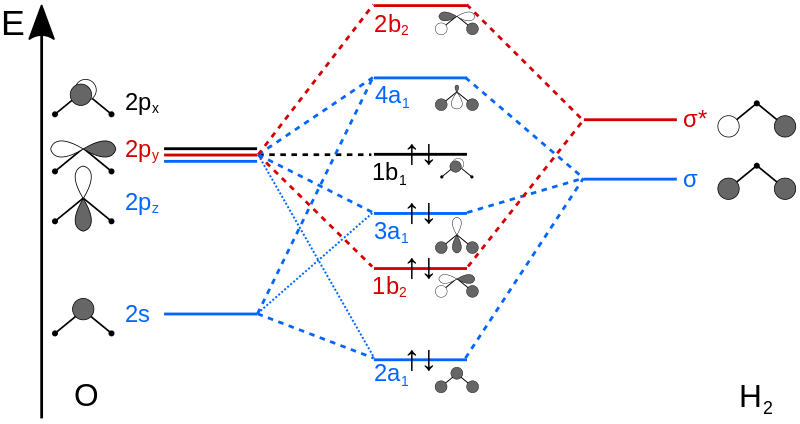
\includegraphics[width = \textwidth]{Atom-ogMolekylefysik/billeder/H2O-MO-Diagram.png}
    \caption{Molekyleorbitaldiagram for vand. Her har de været snedige og anvendt MO'erne for H$_2$-}
    \label{fig:amo:MOvand}
\end{figure}
Bemærk at orbitaler altid skrives med små bogstaver, der afhænger af orbitalens symmetri.

Aufbau princippet gælder også for molekyler, så vand har i grundtilstanden elektronstrukturen:
$$
1a_1^2~2a_1^2~1b_2^2~3a_1^2~1b_1^2~4a_1^2~2b_2^2
$$
Eksponenterne angiver hvor mange elektroner der i hver orbital.
\end{document}